% Preamble
% there are different document classes for books and for presentations
\documentclass{article}
 
\usepackage[utf8]{inputenc}
\usepackage{mathrsfs}
\usepackage{boondox-cal}
\usepackage{amsmath}
\usepackage{graphicx}

\title{Hello world}
\author{Aditya Yadav}
\date{November 2023}

% Actual content starts here 
\begin{document}
\maketitle
\section{Introduction}

\subsection{Writing an Inline Formula}
A formula is inserted between two \$s, like this $e^{\pi i}=-1$

\subsection{Writing a Formula in display mode(centered)}
Insert the formula between two \$\$s, like this $$ \mathcal{L}=\frac{1}{n}\sum_{i=1}^{n}(\hat{y}-y)^2$$

\subsection{Non Autoscaling brackets}
$$(\frac{1}{n}+1)^n$$

\subsection{Autoscaling brackets}
$$\left(\frac{1}{n}+1\right)^n$$

\subsection{Limits}
$$e=\lim_{n\to\infty}\left(\frac{1}{n}+1\right)^n$$

\subsection{$n^{th}$ root}
$$\sqrt[3]{8}=2$$
$$\sqrt[2]{9}=3$$
$$\sqrt[n]{x}=x^{\frac{1}{n}}$$

\subsection{Numbered List of items}
\begin{enumerate}


\item Mean Squared Error Loss 
$$\mathcal{L}=\frac{1}{N}\sum_{i=1}^{n}(\hat{y}-y)^2$$

\item Softmax 
$$P_{y_i}=\frac{e^{y_i}}{\sum_{j=1}^{n}e^{y_j}}$$

\item Cross Entropy Loss
$$\mathcal{L}=\sum_{i=1}^{N}(P_i*log(\frac{1}{Q_i}))$$

\end{enumerate}

\subsection{Unordered List of items}
\begin{itemize}


\item Gradient of Loss wrt to output function
$$\nabla_{y}\mathcal{L}=-\frac{1}{y_l}e(l)$$

\item Gradient of Loss wrt to output layer's pre-activation 
$$\nabla_{a^{L}}\mathcal{L}=\frac{\partial\mathcal{L}}{\partial{y}}*\frac{\partial y}{\partial{a^{L}}}=-(e(l)-y)$$

\item Gradient of Weights between last layer and output layer
$$\nabla_{W^{L}}\mathcal{L}=\frac{\partial\mathcal{L}}{\partial{a^{L}}}*\frac{\partial a^{L}}{\partial{W^{L}}}=-(e(l)-y)*(h^{L-1})^T$$

\end{itemize}

\subsection{Vector dot product}
$$\vec{v}\cdot\vec{w}$$

\subsection{Matrices}

$$
\begin{bmatrix}
1&2&3\\
4&5&6\\
\end{bmatrix}\cdot
\begin{bmatrix}
	a&b\\
	c&d\\
\end{bmatrix}
$$

\subsection{Include Images}
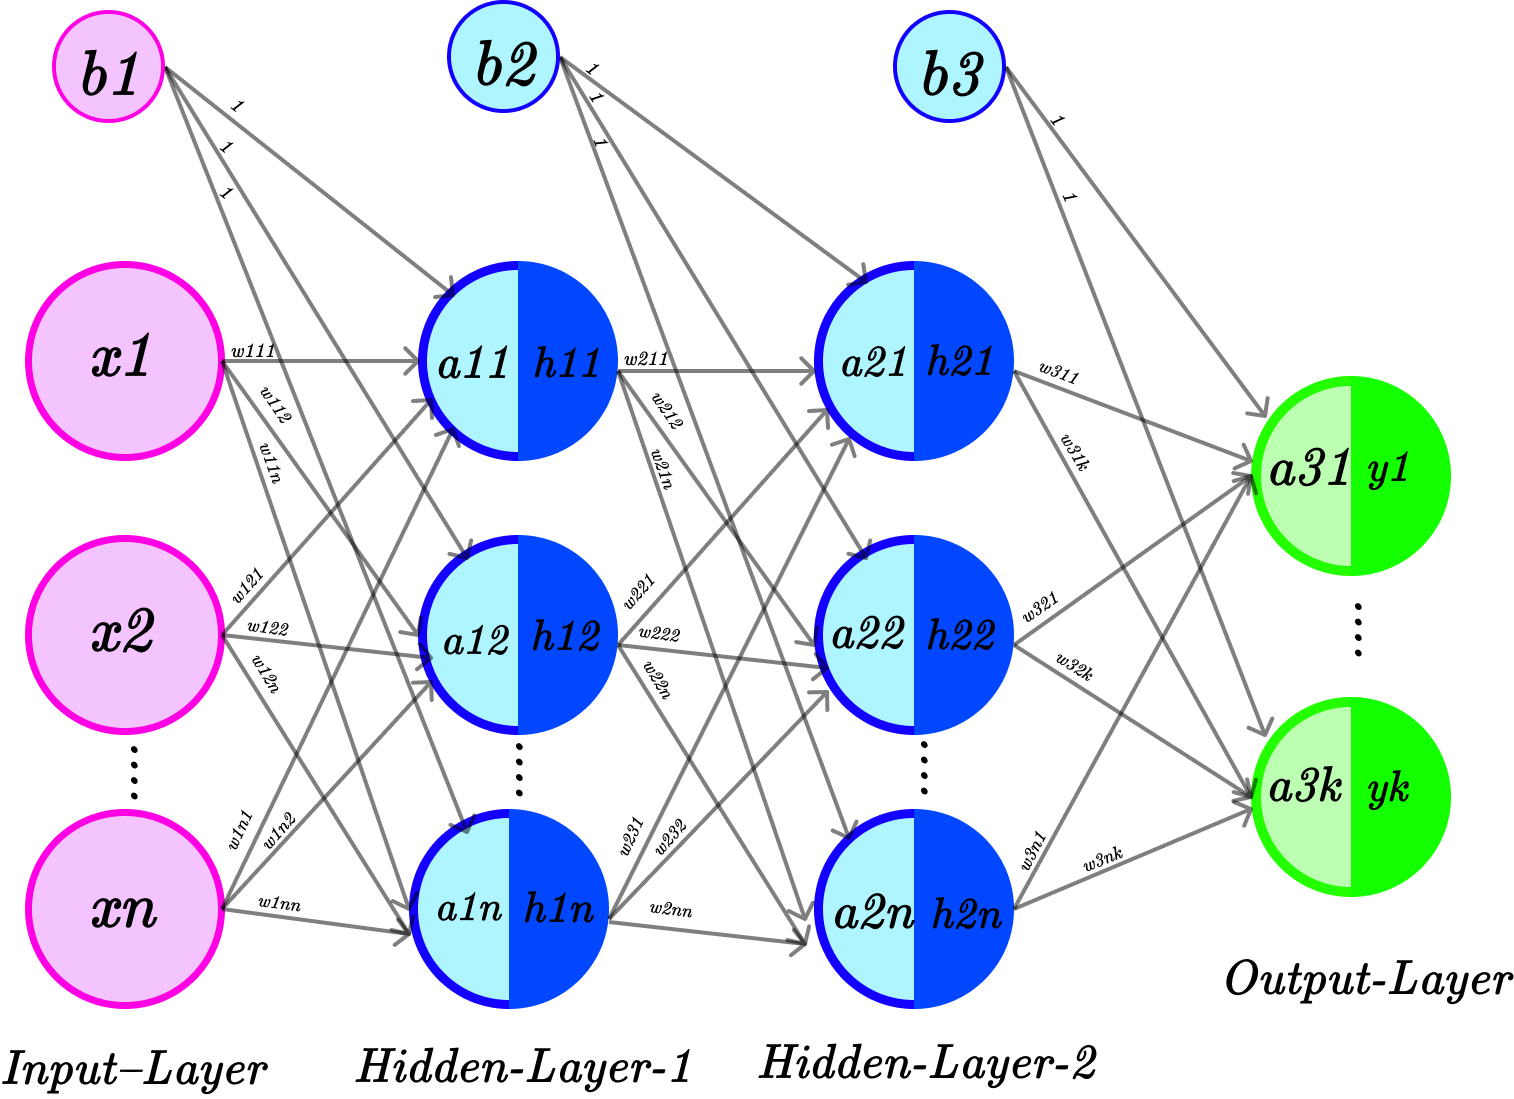
\includegraphics[scale=0.2]{ANN.png}

	


\end{document}

